%課題研究レジュメテンプレート ver. 1.2

\documentclass[uplatex]{jsarticle}
\usepackage[top=20mm,bottom=20mm,left=20mm,right=20mm]{geometry}
\usepackage[T1]{fontenc}
\usepackage{txfonts}
\usepackage{wrapfig}
\usepackage[expert,deluxe]{otf}
\usepackage[dvipdfmx,hiresbb]{graphicx}
\usepackage[dvipdfmx]{hyperref}
\usepackage{pxjahyper}
\usepackage{secdot}

\makeatletter
  \renewcommand{\section}{%
    \if@slide\clearpage\fi
    \@startsection{section}{1}{\z@}%
    {\Cvs \@plus.5\Cdp \@minus.2\Cdp}% 前アキ
    {.5\Cvs \@plus.3\Cdp}% 後アキ
    %{\normalfont\Large\headfont\raggedright}}
    {\normalfont\raggedright}}

  \renewcommand{\subsection}{\@startsection{subsection}{2}{\z@}%
    {\Cvs \@plus.5\Cdp \@minus.2\Cdp}% 前アキ
    {.5\Cvs \@plus.3\Cdp}% 後アキ
    %{\normalfont\large\headfont}}
    {\normalfont}}

  \renewcommand{\subsubsection}{\@startsection{subsubsection}{3}{\z@}%
    {\Cvs \@plus.5\Cdp \@minus.2\Cdp}%
    {\z@}%
    %{\normalfont\normalsize\headfont}}
    {\normalfont}}
\makeatother
%ここから上を編集する必要はない.





\title{\vspace{-14mm}Twitterユーザーの興味とリツイート行為の関係分析}
\author{PMコース 矢吹研究室 1442014 岩橋瑠伊}
\date{}%日付を入れる必要はない.
\pagestyle{empty}%ページ番号は振らない.
\begin{document}
\maketitle





\section{研究の背景}
SNSは,コミュニケーションプラットフォームとして私たちにとって大変身近な存在になっている.同時にどのSNSにビジネスの可能性があるかなどの注目も集まっている.
今回は数あるSNSの中からTwitterを選び,Twitterでの広告などのビジネスをより効果的にする手法について考えていく\cite{sns}.

Twitterは2006年7月15日に開設された「ツイート」と称される140文字以内の短文の投稿を共有するウェブ上の情報サービスである.2015年12月時点で,1カ月の間にTwitterにログインしたアクティブユーザー数は3500万人である.世界全体では3億2000万人で約1割が日本国内からのアクセスである\cite{twitter}.

Twitterでは,ツイートをすると自分のフォロワーの見ているタイムラインに自分のツイートが表示される.逆に,自分がフォローしている人がツイートをすると自分のタイムラインにそのツイートが表示される.その他のTwitterの機能にリツイートがある.リツイートとは,元のツイートのユーザー名のまま自分のフォロワーの見ているタイムラインに転送する機能である.この機能を使うことで自分が興味深い,拡散したいと思ったツイートを自分のフォロワーに伝えられる.

私は自分のタイムラインを読んでいるときに,ユーザーのツイートから判断するにそのユーザーが興味を持っていない内容のツイートに対してリツイートをしている現象を発見した.必ずしもツイートの主旨とそれをリツイートするユーザーのツイートの主旨は類似しないと考えた.

Twitterで商品の広告を行うとすると,興味を持ったユーザーにリツイートされるのが最も効率が良いと考えられる.つまり,興味を持ったユーザーにリツイートされるようなツイートを作れるようにすれば効率よく広告できるようになるだろう.ツイートしたユーザーや主旨の変化でリツイートユーザーが変化しているならば,興味を持ったユーザーにリツイートされやすい状態も見つかるのではないかと考えた.

\section{研究の目的}

ツイート内容,公式アカウントであるか非公式アカウントであるか,フォローフォロワー数等の環境変化の下で,ツイートの趣旨とリツイートユーザーのツイートの趣旨の関係性の変化を明らかにする.

\section{プロジェクトマネジメントとの関連}

ツイートするユーザーや主旨を変えることによってツイートを伝えたいユーザーの範囲を定められるならば,Twitterで広告を行う企業にとってのステークホルダー・マネジメントになると考えられる.

\section{研究の方法}

最低100リツイート以上されているツイートを集め,そのツイートのリツイートユーザーの中からTwitterAPIを利用して100人(TwitterAPI制限の限界値)のユーザーIDとScreanNameを取り出す.

取得した100人のユーザー全員の最新500ツイート(対象ユーザーの総ツイート数が500に満たない場合は対象ユーザーの全てのツイート)をTwitterAPIで取得する.


取得した100人のユーザーのそれぞれ500ツイートをまとめてMeCabで形態素解析を行い,文章中に含まれる名詞に関してtf-idfで重み付けをする.


これにより抽出された名詞をチェックし,一つでもリツイートされたツイートの内容と関連する名詞が確認された場合,そのユーザーはリツイートされたツイートの内容と関係があると判断する.


\section{現在の進捗状況}

図1の3つのツイートを分析をした.ツイートの趣旨とリツイートユーザーのツイートの趣旨の関係性があると見なした人数は,1番では80人,2番では62人,3番では6人となった.次の段落から結果の考察を行う.

Twitterの公式アカウントであるのは1番だけで,2番3番は一般のユーザーである.1番のツイートが最もツイートの趣旨とリツイートユーザーのツイートの趣旨の関係性があると見なされたのは,企業の公式アカウントであるという影響力があったからではないかと考えた.

2番が1番より関係性が弱いのは,一般のユーザーであることが原因だと考える.一般のユーザーは個人がフォローしたいと思ったユーザーをフォローするのに対し,企業の公式アカウントはその企業に興味を持っている人を主にフォローする傾向にある.つまり,企業の公式アカウントは自社の広告の為にフォローするユーザーを厳選しているのである.

3番が非常に弱い関係性となったのは一般のユーザーである事だけではなく,ツイートの内容に原因があったと考える.内容は11月14日にスーパームーンが見られるというものである.珍しい現象が見られるといった内容は,その現象について知らなかったとしてもツイートを見た瞬間にリツイートしがち(私がTwitterを利用した際の経験より)ということから非常に弱い関係性に繋がったのではないかと考える.

\begin{figure}[h]
\centering
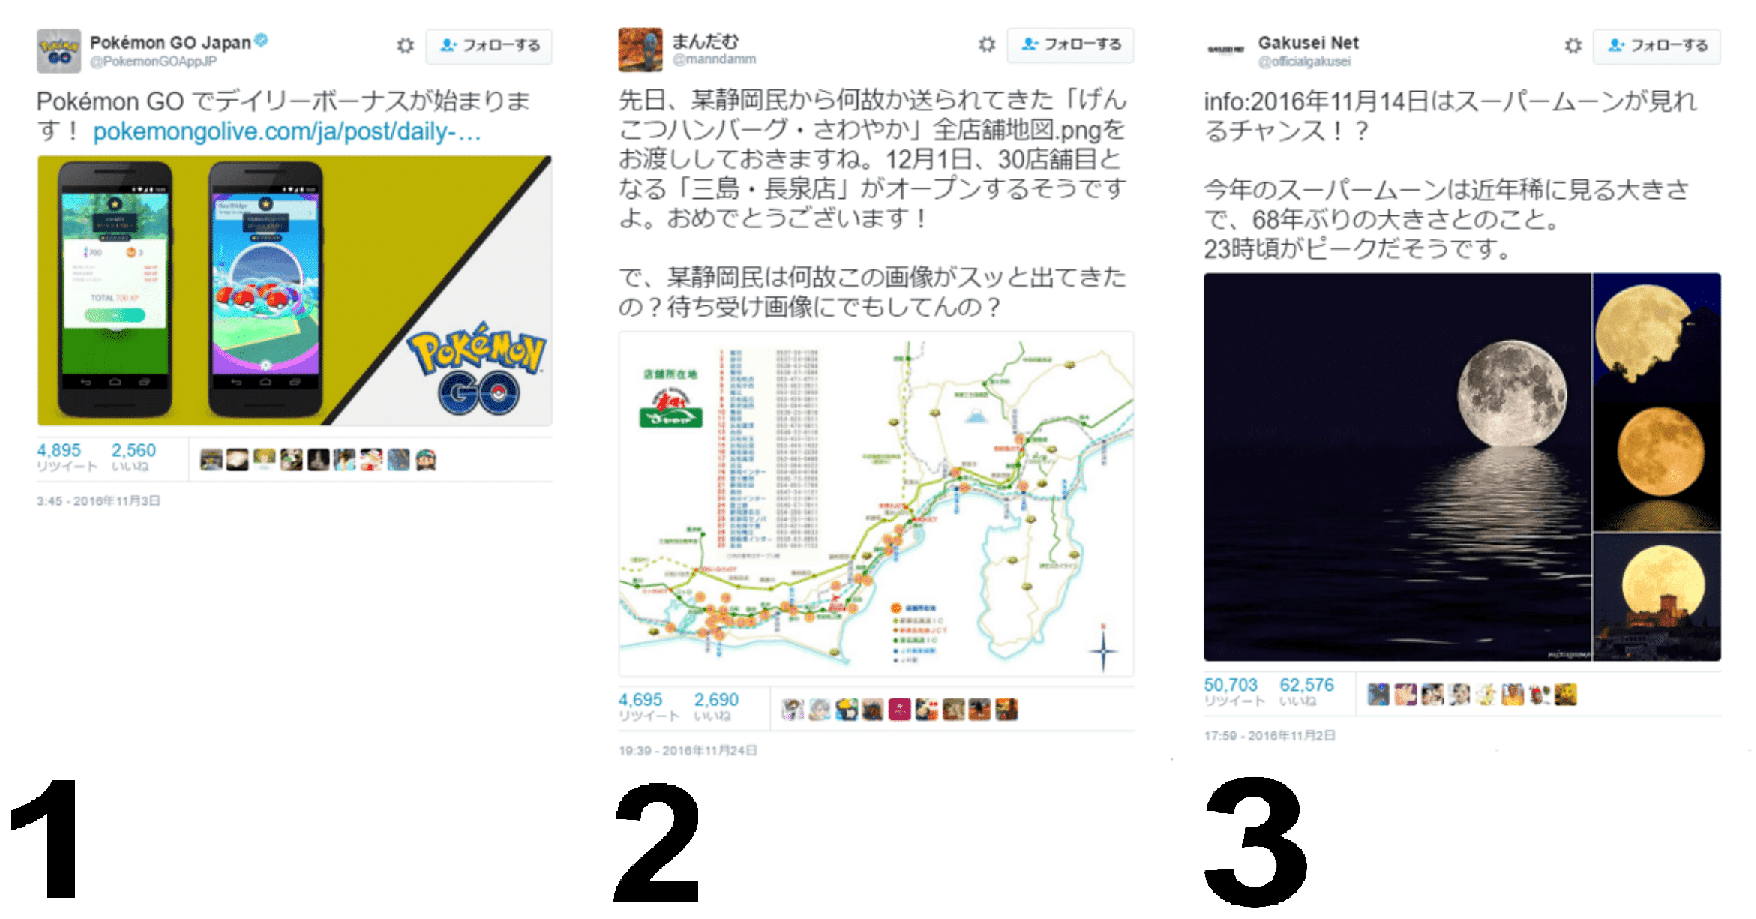
\includegraphics[width=15cm]{g1.pdf}
\caption{リツイートユーザーを分析した3つのツイート\newline 左から1番2番3番とする}\label{ツイート}
\end{figure}

\section{今後の計画}
今後は以下のように研究を進めていく.
\begin{enumerate}
\item まだデータの数が少ないので多くのツイートを分析する.
\item 様々な条件のツイートを分析することで新たな発見をする.
\end{enumerate}

\bibliographystyle{junsrt}
\bibliography{biblio}%「biblio.bib」というファイルが必要.

\end{document}